
\subsection{Инициации перемещения предметов между хранилищами}

\textbf{Участники:}
Менеджер, Администратор, Перевозчик.

\textbf{Описание:}
Менеджер договаривается с Перевозчиком о перевозке груза из 
хранилища А в хранилище Б. Менеджер создает заявку на перемещение
предметов из хранилища А в хранилище Б. Администраторы хранилищ 
А и Б подтверждают либо отклоняют ее.

\begin{figure}[h]
  \centering
  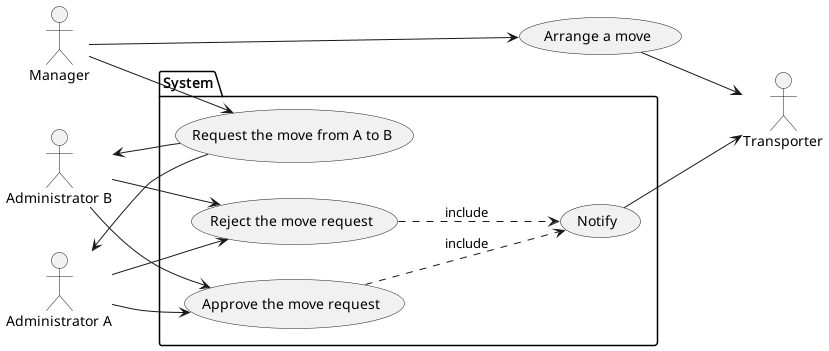
\includegraphics[width=12cm]{../../doc/spec/figure/usecase/move_arrange/Storage Net, Use Case, Move Arrange.png}
  \caption{Use Case: Move Arrange}
\end{figure}

\subsection{Отправление предметов из хранилище}
Аналогично прибытию товаров в хранилище, но наоборот.

\begin{figure}[h]
  \centering
  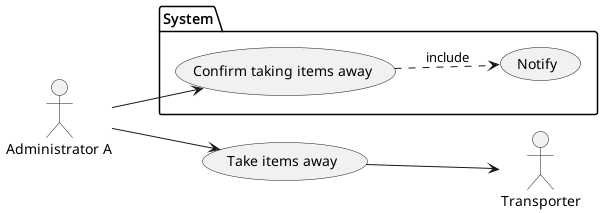
\includegraphics[width=12cm]{../../doc/spec/figure/usecase/move_from_confirm/Storage Net, Use Case, Move from begin.png}
  \caption{Use Case: Move from begin}
\end{figure}

\subsection{Прибытие предметов в хранилище}
Аналогично поставке товаров в хранилище, но с перевозчиком.
